Finding minimal repairs has been shown to be NP-Complete even for FDs only \cite {Chiang}.
Moreover, finding minimal repair for DCs and numerical values only is known to be MaxSNP-hard \cite{Bertossi}.
The work in \cite{XuChu} proposes an approximate holistic algorithm that is capable of generating nearly-optimal repairs for a given set of DCs.
The algorithm we propose for generating sample repairs for DCs is built upon two ideas: first, we try to generate a repair in a holistic manner as proposed in \cite{XuChu}, Second, we uses the
idea of generating random samples from the space of repairs, introduced in \cite{Beskales_sampling}.
Before going into the algorithm specifications, we will first see why the two of the above ideas cannot solve the problem alone.

\subsection{Previous Approaches} \label{sec:previous}
First we will see why the repair sampling approach described in \cite{Beskales_sampling} is not self-sufficient to generate repairs for Denial-Constraints as well.
The idea in \cite{Beskales_sampling} is to grow the set of clean cells by merging the cells belonging to same equivalence class.
It is easy to build equivalence classes in case of FDs and CFDs, in other words when the set of predicates $B = \{ =, \neq\}$; 
but the equivalence class cannot be determined when the predicates are more loose, such as from the set $B = \{ =, \neq\, <, >, \leq, \geq, \approx \}$.

Second, the approximate holistic algorithm in \cite{XuChu}, has two issues due to which it cannot be used for generating repairs.
One, the approximate algorithm uses minimum vertex cover (MVC) to find an approximately minimal repair, but it still does not guarantee to cover all cardinality-Minimal space.
For example, consider the data instance given in  Table \ref{table:eg1}, the MVC for the conflict hyper-edges is set $\{t_1.C, t_2.C, t_4.C\}$.
The holistic algorithm will pick one cell from MVC, say $t_2.C$ and form a frontier set and generates a repair expression for it.
The output repair from this will be the first repair in Table \ref{table:eg2}, i.e. $t_1.C = t_2.C = t_3.C = t_4.C = 5$.
Although the cardinality-minimal repair is the second repair in Table \ref{table:eg2}, i.e. $t_1.C = t_2.C = 3,t_4.D = V \leq 3$.
This cardinality-Minimal repair could have been achieved if the algorithm would have picked up cell $t_4.D$ first (that is not in MVC) and then $t_2.C$ to generate repair, we will show this in detail in Section \ref{sec:algoOver}.

The other issue with the holistic approach is that, it can also generate repairs which are not even Set-Minimal.
The cell modifications governed by the repair expression can generate new violations which are handled in the next iteration of the algorithm.
We will see an example where a series of new violations can end up generating a Not-Set-Minimal repair.
Consider a database instance and a set of DCs as shown in figure \ref{fig:eg4}.
The dotted box represents a violation hyperedge of a conflict hypergraph (CH).
The MVC for a single hyperedge CH can be any cell in that hyperedge.
Say, algorithm selects cell $t_2.B$ as MVC and generates a repair, as shown in Figure \ref{fig:notSetMinEg}(i), but introduces a new violation.
In the next iteration cell $t_2.A$ is a part of MVC and Figure \ref{fig:notSetMinEg}(ii) is the repair with a new violation, and so on, 
Figure \ref{fig:notSetMinEg}(i-iv) shows the repair and new violations introduced at each step of the iteration.
Figure \ref{fig:notSetMinEgFinal} shows all the cells changed in the repair process.
Now observe that the value of cell $t_2.B$ can be reverted back to its original value 5, and the resulting repair is shown in Figure \ref{fig:notSetMinEgOther} which is still a valid repair.
This proves that the holistic data cleaning algorithm can generate repairs which are not Set-Minimal.

\begin{figure}
   \centering
   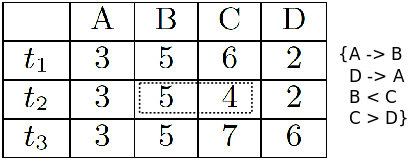
\includegraphics[scale=0.25]{eg4.png}
   \caption{Unclean database instance and a set of DCs. Dotted line is a hyperedge, showing violation.}
   \label{fig:eg4}
\end{figure}

\begin{figure}
   \centering
   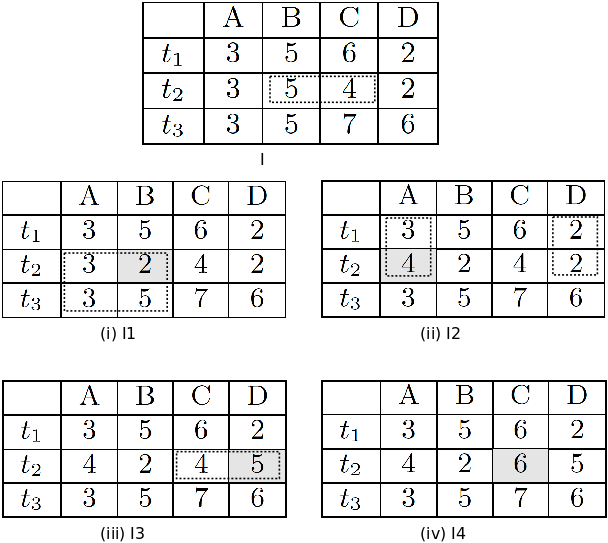
\includegraphics[scale=0.28]{notSetMinEg.png}
   \caption{Shows the repaired cell at each iteration and the new violation.}
   \label{fig:notSetMinEg}
\end{figure}

\begin{figure}
   \centering
   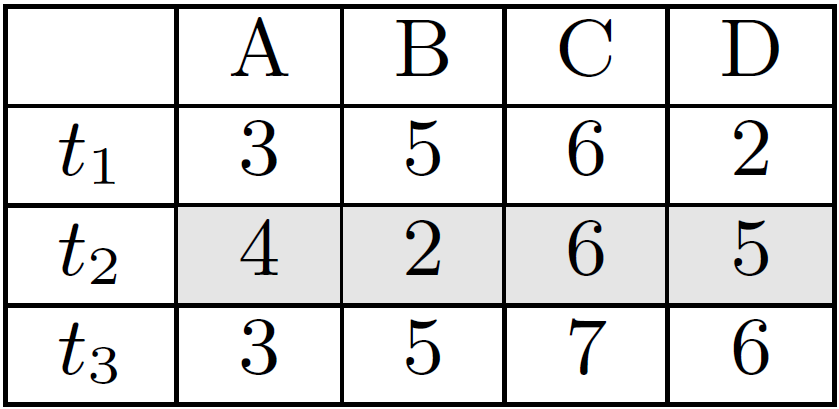
\includegraphics[scale=0.2]{notSetMinEgFinal.png}
   \caption{All the cell changed with respect to original I.}
   \label{fig:notSetMinEgFinal}
\end{figure}

\begin{figure}
   \centering
   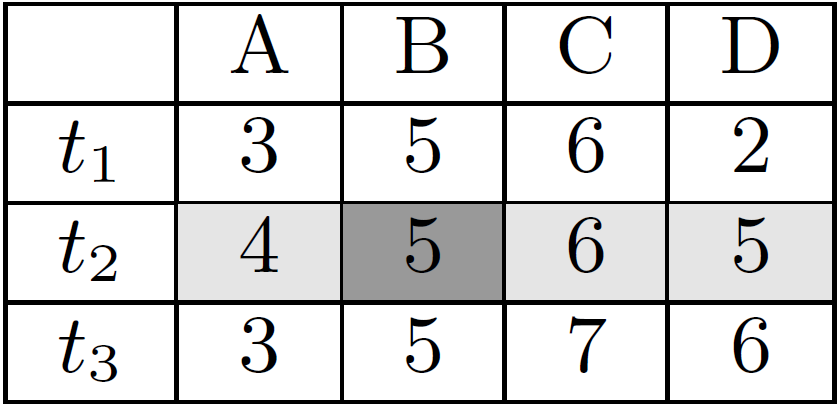
\includegraphics[scale=0.2]{notSetMinEgOther.png}
   \caption{Value of Cell $t_2.B$ can be reverted and the repair is still valid.}
   \label{fig:notSetMinEgOther}
\end{figure}

%
%\begin{table} \label{tab:eg1}
%\centering 
%\begin{tabular}{|c|c|c|c|c|}  \hline
%      & A & B & C & D 	\\ \hline
%   $t_1$ & 3 & 5 & 6 & 2 	\\ \hline
%   $t_2$ & 3 & 5 & 4 & 2 	\\ \hline
%   $t_3$ & 3 & 5 & 7 & 6 	\\ \hline
%\end{tabular}
%\caption{Sample Data.}
%\end{table}
%
%
%
%
%
%
%\begin{table} \label{tab:eg1}
%\centering 
%\begin{tabular}{|c|c|c|c|c|}  \hline
%      & A & B & C & D 	\\ \hline
%   $t_1$ & 3 & 5 & 6 & 2 	\\ \hline
%   $t_2$ & 3 & \cellcolor[gray]{0.9}2 & 4 & 2 	\\ \hline
%   $t_3$ & 3 & 5 & 7 & 6 	\\ \hline
%\end{tabular}
%\caption{Sample Data.}
%\end{table}
%
%\begin{table} \label{tab:eg1}
%\centering 
%\begin{tabular}{|c|c|c|c|c|}  \hline
%      & A & B & C & D 	\\ \hline
%   $t_1$ & 3 & 5 & 6 & 2 	\\ \hline
%   $t_2$ & \cellcolor[gray]{0.9}4 & 2 & 4 & 2 	\\ \hline
%   $t_3$ & 3 & 5 & 7 & 6 	\\ \hline
%\end{tabular}
%\caption{Sample Data.}
%\end{table}
%
%\begin{table} \label{tab:eg1}
%\centering 
%\begin{tabular}{|c|c|c|c|c|}  \hline
%      & A & B & C & D 	\\ \hline
%   $t_1$ & 3 & 5 & 6 & 2 	\\ \hline
%   $t_2$ & 4 & 2 & 4 & \cellcolor[gray]{0.9}5 	\\ \hline
%   $t_3$ & 3 & 5 & 7 & 6 	\\ \hline
%\end{tabular}
%\caption{Sample Data.}
%\end{table}
%
%\begin{table} \label{tab:eg1}
%\centering 
%\begin{tabular}{|c|c|c|c|c|}  \hline
%      & A & B & C & D 	\\ \hline
%   $t_1$ & 3 & 5 & 6 & 2 	\\ \hline
%   $t_2$ & 4 & 2 & \cellcolor[gray]{0.9}6 & 5 	\\ \hline
%   $t_3$ & 3 & 5 & 7 & 6 	\\ \hline
%\end{tabular}
%\caption{Sample Data.}
%\end{table}
%
%\begin{table} \label{tab:eg1}
%\centering 
%\begin{tabular}{|c|c|c|c|c|}  \hline
%      & A & B & C & D 	\\ \hline
%   $t_1$ & 3 & 5 & 6 & 2 	\\ \hline
%   $t_2$ & \cellcolor[gray]{0.9}4 & \cellcolor[gray]{0.9}2 & \cellcolor[gray]{0.9}6 & \cellcolor[gray]{0.9}5 	\\ \hline
%   $t_3$ & 3 & 5 & 7 & 6 	\\ \hline
%\end{tabular}
%\caption{Sample Data.}
%\end{table}
%
%\begin{table} \label{tab:eg1}
%\centering 
%\begin{tabular}{|c|c|c|c|c|}  \hline
%      & A & B & C & D 	\\ \hline
%   $t_1$ & 3 & 5 & 6 & 2 	\\ \hline
%   $t_2$ & \cellcolor[gray]{0.9}4 & \cellcolor[gray]{0.6}5 & \cellcolor[gray]{0.9}6 & \cellcolor[gray]{0.9}5 	\\ \hline
%   $t_3$ & 3 & 5 & 7 & 6 	\\ \hline
%\end{tabular}
%\caption{Sample Data.}
%\end{table}
%

\subsection{Algorithm Overview} \label{sec:algoOver}
The algorithm we propose is inspired from the holistic data cleaning algorithm of \cite{XuChu}, with two major modifications.
One, we introduce randomness in selecting an hyperedge and a cell in an hyperedge, where as \cite{XuChu} used minimum vertex cover to select cells to start the repair.
The random selection of cells help us to generate Cardinality-Minimal repairs as well.
Second, we have put restrictions on which cells can be included in the frontier set. 
For each of the randomly picked cell, we do one step look-ahead and check if the cell can produce further violations.
If yes, we mark that cell "unsafe" and choose another cell from the edge.
In Section \ref{sec:previous} we saw that if the a repair is introducing new violations then we can get into a sequence of violations that can result into a Not-Set-Minimal repair.
Therefore, the insight behind the constrained selection of cells is to avoid a sequence of repairs which can end up in a Not-Set-Minimal repair.

We represent the violations in the database instance using hyperedges, similar to \cite{XuChu,Kolahi}.
After all the violations have been detected we get a set of hyperedges, and the graph induced by them is called a \textit{Conflict Hypergraph (CH)}.
It is an undirected hypergraph with a set of nodes P representing the cells and a set of annotated hyperedges E representing the relationships among cells violating a constraint.
More precisely, a \textit{hyperedge} is a set of violating cells from which one of them must change to repair the constraint, and contains: 
(a) the constraint $c$, which induced the conflict on the cells; (b) the list of nodes involved in the conflict.

Consider the example database instance given in Table \ref{table:eg1} and the following set of DCs $\{ A \rightarrow C, B \rightarrow C, R[D=5] \rightarrow R[C=5], C \geq D \}$.
Figure \ref{fig:ch} represents a conflict hypergraph of the present state of the database violations w.r.t the given DCs.
Each hyperedge in the graph contains only the violating cells, and in order to repair it, at least one of its cells must get a new value.
We start our algorithm by picking an hyperedge at random and a random cell within that edge.
Algorithm assumes that this cell needs to be changed and hence identify all the other cells that are involved in the repair of this cell.
This starting set of newly identified cells is called \textit{frontier}.
We call \textit{repair expressions} the list of constant assignments and constraints among the frontier.
Similar to \cite{XuChu}, the frontier and the repair expressions form a \textit{Repair Context} (RC).
Once we are done with the repair context of the first chosen cell, we \textit{freeze} all the edges which got repaired using that RC.
By freeze, we mean that the cells belonging to those edges, if encountered in the frontier of any other RC later, cannot be changed.
If there are more edges remaining in the hypergraph, our algorithm again chooses a remaining hyperedge at random and chooses a cell that is not marked \textit{freeze} from that edge,
and forms the RC for this new cell in the similar fashion.
The algorithm continues till there are no more hyperedges left in the graph.

For example, consider the DCs and hypergraph in Figure \ref{fig:ch}.
Lets say, the algorithm starts by choosing Edge $e4$ and cell $t_4[D]$.
The repair expression for this is simple, i.e. $t_4[D] \leq 3$, so we will assign a fresh value to it, call it $FV$ and cell $t_4[C]$ will be marked \textit{freeze}.
Then we move onto choose the next edge, say this time we choose edge $e2$ and cell $t_2[C]$.
If we have to change $t_2[C]$ then the cell $t_3[C]$ in edge $e2$ should be changed, this gives us the expression $t_2[C] = t_3[C]$.
Cell $t_2[C]$ is related to edges $e1$ as well, and we get the expression $t_2[C] = t_1[C]$.
Cell $t_2[C]$ is related to edges $e4$ as well, and we get the expression $t_2[C] = t_4[C] = 3$, remember that cell $t_4[C]$ is frozen and cannot be changed.
The cell $t_1[C]$ is in edge $e5$ as well, hence the relation for cell $t_1[C]$ will be $t_1[C] \geq 3$.
Therefore the overall repair expression becomes $t_2[C] = t_1[C], t_2[C] = t_3[C], t_2[C] = t_4[C], t_4[C] = 3 $and $t_1[C] \geq 3$.
The cells and their new values will be: $t_2[C] = 3, t_1[C] = 3$ and $t_4[D] = FV$.

Notice that, the repair we obtained above is same as the second repair shown in Table \ref{table:eg2}, which is actually a Cardinality-Minimal repair.
This indicates that the randomized selection of cells is capable of generating Cardinality-Minimal repairs also.

\textbf{Proposition:} Randomized selection of cells guarantee to cover Cardinality-Minimal repairs also. \\
\textit{Proof Sketch:} There are exponential number of repair expressions possible in a single CH depending upon the cell we start with.
Also, each repair expression has different satisfiability with different cardinality.
By using random selection we are allowing all the possible repair expressions, some of which will be Cardinality-Minimal.


\begin{figure}
   \centering
   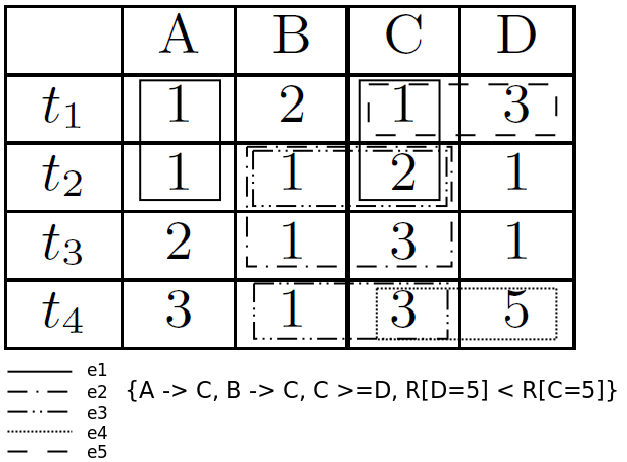
\includegraphics[scale=0.22]{ch.png}
   \caption{Conflict hypergraph.}
   \label{fig:ch}
\end{figure}

Now we will see an example where we demonstrate a constrained selection of cells to limit the space of repairs to Set-Minimal.
Consider the unclean database instance in Fig. \ref{fig:eg4}, cell $(t_2[B], t_2[C])$ forms the only edge in the CH.
We can either choose cell $t_2[B]$ or $t_2[C]$, notice that choosing $t_2[B]$ resulted into a new violation, see Fig. \ref{fig:notSetMinEg}(i).
Hence it is called an "unsafe" cell and will not be chosen.
To check if the cell is "unsafe" we use a one step look-ahead, 
i.e. we assume that the cell has been modified according to the DETERMINATION step and construct a new conflict hypergraph, if that cell introduces a new hyperedge then we mark it "unsafe".
Whereas, in the same example if we select cell $t_2[C]$, the result of DETERMINATION step will be $t_2[C] > 5$ and it will not create a new violation.
This observation leads to the following proposition.

\textbf{Proposition:} A repair context that does not introduce new violations will provide a Set-Minimal repair. \\
\textit{Proof Sketch:} If DETERMINATION step is using a Cardinality-Minimality or Distance-Minimality methods to satisfy the expression, then all the cell changes are minimal and necessary.
Therefore, if we avoid any new violations then the cell changes suggested by the DETERMINATION step are the necessary changes.
Hence, the repair will be Set-Minimal.
